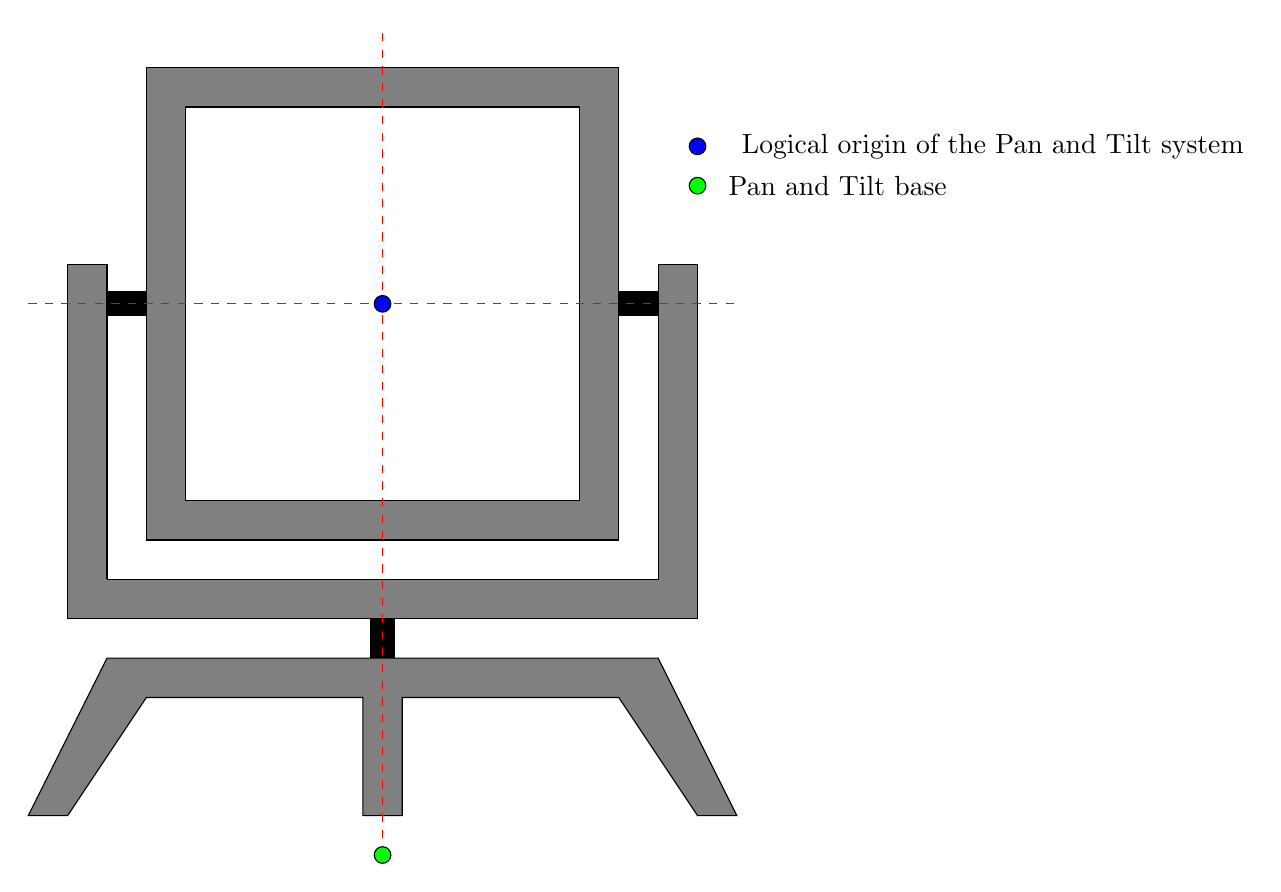
\begin{tikzpicture}[scale=1]

\draw[fill = gray] (0.5,1)--(6.5,1)--(6.5,7)--(0.5,7)--(0.5,1);
\draw[fill = white] (1,1.5)--(6,1.5)--(6,6.5)--(1,6.5)--(1,1.5);

\draw[fill = black] (0,3.85)--(0.5,3.85)--(0.5,4.15)--(0,4.15)--(0,3.85);
\draw[fill = black] (6.5,3.85)--(7,3.85)--(7,4.15)--(6.5,4.15)--(6.5,3.85);

\draw[fill = gray] (0,0.5)--(7,0.5)--(7,4.5)--(7.5,4.5)--(7.5,0)--(-0.5,0)--(-0.5,4.5)--(0,4.5)--(0,0.5);

\draw[fill = black] (3.35,0)--(3.65,0)--(3.65,-0.5)--(3.35,-0.5)--(3.35,0);

\draw[fill = gray] (0,-0.5)--(7,-0.5)--(8,-2.5)--(7.5,-2.5)--(6.5,-1)--(3.75,-1)--(3.75,-2.5)--(3.25,-2.5)--(3.25,-1)--(0.5,-1)--(-0.5,-2.5)--(-1,-2.5)--(0,-0.5);

\draw[dashed, red] (-1,4)--(8,4);
\draw[dashed, red] (3.5,-3)--(3.5,7.5);

\draw[fill = blue] (3.5,4) circle (3pt);
\draw[fill = blue] (7.5,6) circle (3pt);
\draw (11.25,6)node{Logical origin of the Pan and Tilt system};

\draw[fill = green] (3.5,-3) circle (3pt);
\draw[fill = green] (7.5,5.5) circle (3pt);
\draw (9.28,5.5)node{Pan and Tilt base};

\end{tikzpicture}